\chapter{MR-Cube 实现分析}

本章节中将对 \cite{nandi2011distributed} 中提出的 MR-Cube 进行具体分析,包括它的主要贡献和存在的不足。

\section{数据集}

在接下来的章节中需要数据集作为例子,因此首先介绍作为例子的数据集,这里使用\cite{nandi2011distributed}  中的数据集。数据集的表结构如图 \ref{dataset_table} 所示。表中数据记录的是不同地区的用户的查询记录。属性id为表的主键,记录每条记录的id;time为查询时间;uid为用户的id。表中剩余的 6 个属性为维属性,分别是 country,state,city,topic,category,subcategory。country,state,city 记录地区信息,topic,category,subcategory 记录查询内容。其中\textless country, state, city\textgreater 是具有层次型的,同理\textless topic, category, subcategory\textgreater 也是具有层次性的。因此在 GroupBy 时,GroupBy(country, state, topic) 和 GroupBy(state, topic)是等价的。并且不会出现 GroupBy(country, city, topic) 这样的跨越层次的操作。

该数据集对应的 lattice 如图 \ref{dataset_lattice} 所示。图中的 ``*" 表示不需要聚合的属性。因为数据集具有层次型,因此lattice与上一章中看到的有所不同。上一章中提到,若有 D 个维属性,则 lattice 中有${2}^{D}$ 个节点,但由于这个数据集具有层次型,因此节点数有所减少。例如对于 (country, state, city) 这3个属性的 GroupBy,仅有 3 种结果,即 GroupBy(country),GroupBy(country, state)(或 GroupBy(state)) 以及 GroupBy(country, state, city)(或 GroupBy(city))。因此该数据集对应的lattice中共有16个region,也就是该数据集共有16种 GroupBy 类型。


\begin{figure}[!htb]
\centering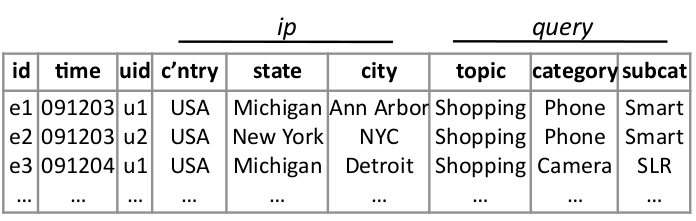
\includegraphics[width=3.5in]{picture/ch_datacube_mr/dataset_table} 
\caption{数据集的表结构}\label{dataset_table} 
\end{figure} 

\begin{figure}[!htb]
\centering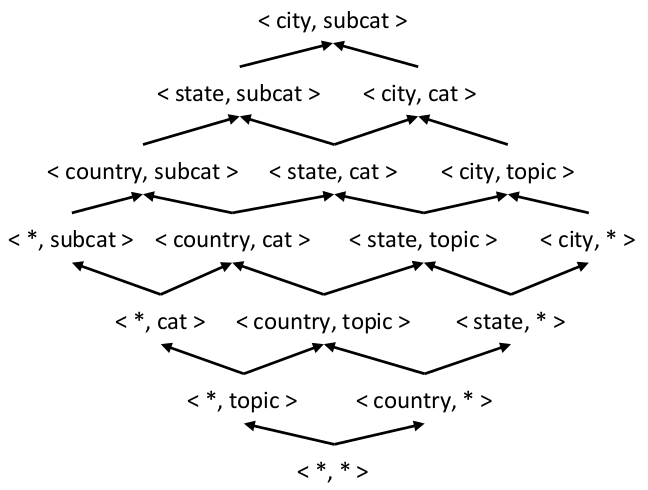
\includegraphics[width=3in]{picture/ch_datacube_mr/dataset_lattice} 
\caption{数据集的lattice}\label{dataset_lattice} 
\end{figure} 

\section{Naive 算法}

算法 \ref{naive_algorithm} 为使用 MapReduce 计算数据立方的 Naive 实现。例如上述的数据集共有16个 region,那么对于输入的每一条记录,将其映射成对应的所有 group,并且与度量属性的值组成 key-value 作为 mapper 的输出。相同 key 值的数据将分派到同一个 reduce 函数中,也即相同 group 值的数据被分派到同一个 reduce 函数中,再进行聚合计算。例如输入的一条记录为 (e1, 091203, u1, USA, New Youk, NYC, Shopping, Phone, Smart),度量函数为 COUNT(DISTINCT(uid)),该度量函数是计算group内有多少不同的uid。那么对于每一条记录,map 都输出 16 个 ([group value], [uid]) 的key-value,分别为([*,*], [u1]), ([*,Smart], [u1]), ([USA, *], [u1])等等。reducer 再对同一个 group 内的数据进行聚合计算。

{\renewcommand\baselinestretch{1} 
\begin{algorithm}[!ht]
\caption{Naive Algorithm}
\label{naive_algorithm}
{\fontfamily{\familydefault}\selectfont

	\begin{algorithmic}[1] %每行显示行号
    \Function {MAP}{e}
    	\State e is a tuple in the dataset
        \ForAll {Region R in C}
        	\State k=R(e)
        	\State EMIT([k], [e])
        \EndFor
   	 \EndFunction
     \State
     \Function {REDUCE}{k,$\left\{ e1,e2,...\right\}$}
     	\State let M be measure function
        \State EMIT(k, M($\left\{ e1,e2,...\right\}$))
     \EndFunction
	\end{algorithmic}
}
\end{algorithm}
\par}

Naive的方法实现起来非常简单,对于较小的数据集也有很好的效果,但是随着数据集规模的增大,Naive方法的不足则非常明显,主要包括以下两个方面。

\begin{itemize}

\item \textbf{中间数据过多}

若 lattice 中的 region 数量为 $|C|$,数据集的大小为 $|D|$,则中间数据的数据量为 $|C|\times |D|$。随着维属性数量的增加,与层次的加深,中间数据的数据量则会巨增,必然导致 map 阶段有大量的磁盘 I/O,以及 shuffle(sort) 阶段有大量的数据需要排序,对整体的效率有非常大的影响。

\item \textbf{超大group}

在 MapReduce 计算中,总体的计算时间是由计算时间最长的 reducer 决定。因此若各个 reducer 分配到的要计算的数据量差异较大时,会导致某些 reducer 运行时间远大于其他 reducer。 在 Naive 的计算方法中,具有相同 group 值的数据会在一个 reducer 中计算,当一个 group 很大时,例如 lattice 中处于底层的 region 中的 group 相对就会较大,它运行的时间就会很长,而其他处理小 group 的 reducer 因为较早处理完数据,可能会空闲等待,甚至重新启动大 group 的计算,但重启计算效果往往并不佳,最终导致整个 MapReduce 的计算时间过长。

\end{itemize}

以上两个不足,主要出现在整体性度量函数的计算中,而对于代数度量函数,例如SUM,COUNT,AVG 等,则不会有以上的问题。因为MapReduce的combiner机制与代数度量函数的计算有非常好的整合。combiner 是 MapReduce 一个重要的机制,它等同于本地的 reducer。它会对 mapper 的输出进行一次本地的 reduce 计算,然后再将数据发到相应的 reducer 上,这样可以减少网络传输的数据量和reducer 的计算量。正因为这个 combiner 的作用,对于代数度量函数,combiner 可以在本地对同一个 group 内的数据进行一次计算,将一个 mapper 上同一个 group 内的数据压缩成一条记录发送给 reducer,而不是将这个 group 内的数据直接发送到 reducer上,这样每个 reducer 获得的数据量比不使用 combiner 获得的数据量要少得多。由于mapper的数量是有限的,那么分发到一个reducer上一个group内的数据也是有限的。这样有限的数据必然不会导致中间数据过多和各个reducer上数据的不均匀。实验部分也会对这两种度量进行比较。

但是对于整体性度量函数,combiner的作用却可能很小,这也是整体性度量函数与代数度量函数最大的区别,因为整体性度量函数中间结果的数据量是不确定的。例如对于COUNT(DISTINCT(uid))的计算,combiner可将同一个group内多条具有相同uid的记录压缩成一条输出,若uid取值较多,甚至无重复,则combiner几乎无法发挥作用。那么就会出现以上提到的两个问题。针对这两个问题,MR-Cube提出了相应的解决方案。

\section{MR-Cube}

\subsection{整体性度量的划分}

对于大 group 的问题,可以将一个大 group 划分成多个子 group,将这些子 group 分发到多个 reducer 上计算,即可解决 reducer 计算数据量不均匀的问题。

对于代数度量函数,数据是可以随意划分的。但是整体性度量函数的划分就没有这么简单了。例如整体性度量函数 COUNT(DISTINCT(uid)),它是计算不同的 uid 的数量。如果对数据集进行随意的划分,每个子块的计算结果是不同的 uid 列表,即对子块中相同的uid只保留一个。然后再对这些 uid 列表进行统计计算 COUNT(DISTINCT(uid))。这里每个子块的计算结果不能是COUNT(DISTINCT(uid)),这样会导致最终结果是错误的。中间结果是不同的 uid 列表,如果 uid 重复度非常高,那么各个列表中uid的数量较少,这种划分计算方法是可行的。但倘若 uid 的重复度非常低,各个列表的uid很可能跟子块中uid数量同样多,那么这种随意划分的方法则毫无作用。 

因此 MR-Cube 的论文中给出了一种对整体性度量函数进行划分的方法,称为部分代数度量 (Partially Algebraic Measure)。例如对于 COUNT(DISTINCT(uid)) 的度量计算,数据可按照 uid 进行划分,那么具有相同 uid 的记录会被划分到同一个子块中,而每个子块之间的 uid 是不会有相同的。这样对于每个子块都可以输出一个整数,即该子块 COUNT(DISTINCT(uid)) 的结果,最后将各个子块的结果相加即可得到最终结果。论文中将 uid 这样的用来划分的属性称之为代数属性。这样的划分方式对于很大部分的整体性度量都是有效的,例如TopK,MODE等。


\subsection{Reducer-Unfriendly Group}

确定了数据的划分方法,下一个问题是哪些 group 需要划分,也就是哪些 group 是较大的 group。在论文中使用了随机均匀采样的方式选取部分的数据进行数据立方的计算,在每个 group 内做 COUNT,也就是统计每个 group 的大小,然后根据数据集大小、采样数量、reducer limit(根据内存大小估算reducer可处理的数据量)以及使用切诺夫界确定一个 group 是否是 reducer-unfriendly group。用直观的理解即是,通过概率统计的方式确定采样中的 group 是否是较大的 group,这些 group 被称为 reducer-unfriendly group。并且对于 unfriendly 的 group,会根据group的大小以及reducer limit 估算出划分因子。对于划分因子的直观理解,即是这样一个大 group 应该划分多少子块,才能令每个子块不超过 reducer 处理数据量的上限。

若一个 region 中有一个 group 是 reducer-unfriendly 的,那么这个 region 也就是 reducer-unfriendly 的。在采样后的正式计算中,对于 reducer-unfriendly region 内的所有 group 都需要进行划分。划分的方式使用上一节中提到的对整体性度量的划分方式,即根据某一个代数属性,如 uid 进行划分。如图\ref{region_partition}所示,根据采样的结果将region划分成了 friendly 和 unfriendly 两类。对于 unfriendly 的 region,region 内的所有 group 都需要划分,论文中使用求余方式进行划分。

\begin{figure}[!htb]
\centering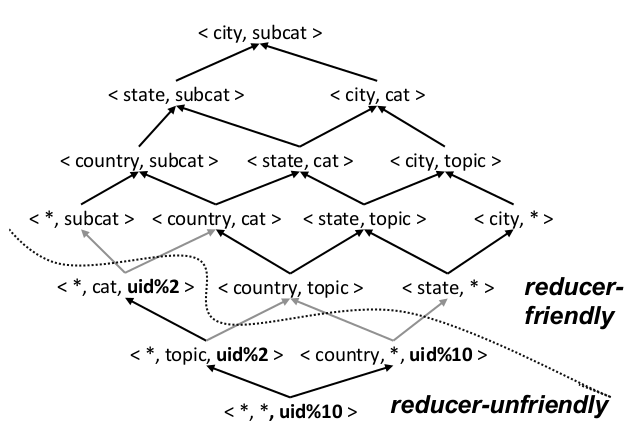
\includegraphics[width=3.5in]{picture/ch_datacube_mr/region_partition} 
\caption{根据uid被划分的lattice}\label{region_partition} 
\end{figure} 

上述的方法只记录需要划分的region,这是因为 region 的数量远比 group 少得多。若要记录所有的需要划分的 group,则需要太大的开销。只记录region的方法能保证大 group 的划分,但是如果 region 中只有 1 个 group 是 unfriendly 的,其他的friendly 的 小group 也要被迫划分,这样将导致不必要的划分以及出现过多的被划分数据,加重了最后的合并操作。同时,论文中使用了求余的方式进行划分,这样的哈希方式非常简单,在很多情况下也是有效的,但是在一些情况下,也可能导致划分的不均匀。就这两点不足,这样的划分方式仍有可改进的空间。

\subsection{Batch Area}

对于Naive方法中的另一个问题,中间数据过多的问题,MR-Cube中提出了 Batch Area 的概念。也就是利用 region 之间的父子关系,将多个 group 放在同一个 reduce 函数中计算,而不是像 Naive 的方法,一个 reduce 函数只计算一个 group。论文中给出了划分 batch 的一些规则,规则包括以下几点。
\begin{itemize}\setlength{\itemsep}{0pt}
\item reducer-unfriendly 的 region 和 reducer-friendly 的 region 不可划分在同一个batch内。
\item 对于 Reducer-unfriendly region 的划分,同一个 batch 内的 region 需要有相同的划分因子。
\item 同一个 batch 中的 region 需要有父子关系。
\item 两个 batch 的 region 数量差别不能超过2。
\end{itemize}

图\ref{batch_area}是其中一种合乎规则的划分方式。图中使用虚线将各个batch加以划分。

\begin{figure}[!ht] 
\centering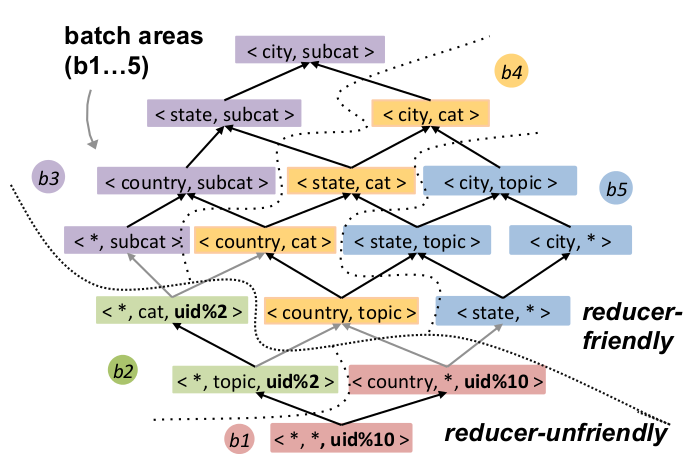
\includegraphics[width=3.5in]{picture/ch_datacube_mr/batch_area} 
\caption{Batch Area}\label{batch_area} 
\end{figure}

对于同一个 batch 内的 group 要如何计算有很多方法,论文使用的是BUC,(bottom up cubing algorithm)。但这种方法需要对数据扫描多次,而 Mapreduce 的 reducer 中提供的迭代器仅能对数据扫描一次,若要对数据进行多次扫描,则需要载入内存中。并且 BUC 这种方法也未充分利用 Mapreduce 框架的特性,例如排序功能。因此这里可以考虑替换其他的方法。同时,论文中只给出了batch 划分的规则,提到可用枚举、局部贪心或者模拟退火的方式找出合乎规则的 batch,并没有给出具体的方法,而模拟退火这样的计算方法又稍微复杂。因此这里可以考虑提出简单而有效的划分方法。


\section{贡献与不足}

MR-Cube \cite{nandi2011distributed} 这篇论文对使用 Naive 算法计算整体性度量函数的数据立方中存在的问题提出了一些非常有效的改善方法,论文的主要贡献包括:

\begin{enumerate}
\item 提出了对整体性度量划分的方法。
\item 提出了如何判断 group 是否需要划分,以及其划分的方法。
\item 提出了将多个 group 合并一起计算的 batch area 的概念。
\end{enumerate}

但是以上的方法也存在一些问题。

\begin{enumerate}
\item 论文中通过 region 内的一个大 group 将一个 region 内的所有 group 都贴上 reducer-unfriendly 的标签,导致 region 内所有的 group 都要划分。有些情况下可能一个 region 就只有一个大 group,而其他的 group 都很小,这样就导致了不必要的划分和加重后续的合并操作。
\item 论文中使用求余(\%)方法对数据进行划分,求余是一种哈希方法,但是这种哈希方法在一些情况下,可能会导致划分的不均匀。
\item Batch area 内的计算,也就是多个 group 之间的计算,论文里使用的 BUC 的方法,虽然这种方法很合适有阈值限定的情况(例如 HAVING),但是它需要对数据进行多次扫描,并且没有很好地利用 Mapreduce 本身的一些优势,例如排序。
\item 论文中只给出了 batch area 的规则,并没有提供简单且能满足规则的划分方法。
\end{enumerate}

针对以上4点,本论文提出了 TSP-Cube,将Tera-Sort、Pipesort 与数据立方的计算相结合,从而改进对 MR-Cube 的不足。





